\chapter{PLANTEAMIENTO DEL PROBLEMA}
\section{Descripción de la Realidad Problemática}

En la era digital actual, el consumo de contenido audiovisual en redes sociales ha crecido exponencialmente, convirtiéndose en una fuente invaluable de información y entretenimiento. 
Una de los principales viene a ser la búsqueda de la actualidad del mundo, de acuerdo a una encuesta realizada por Pew Reasearch Center al sector adulto de EEUU, 3 de cada 10 adultos utilizan regularmente Youtube como plataforma de noticias, siguiendo Instagram y Tiktok. La cantidad de información que se genera día a día es abrumadora y el tiempo escaso.

\begin{figure}[h]
	\centering
	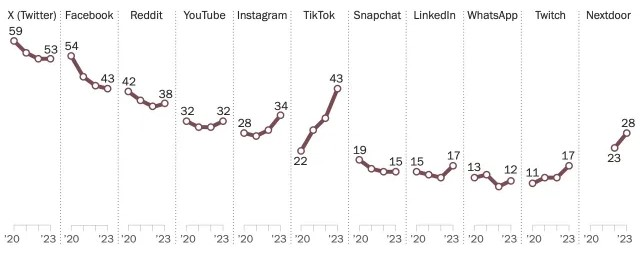
\includegraphics[width=0.80\textwidth]{1/figures/Tendencias_Redes_2023.jpg}
	\caption[Porcentaje de usuarios en base a su consumo de noticias en redes sociales en 2023]{Porcentaje de usuarios en base a su consumo de noticias en redes sociales en 2023. \\ Fuente: \cite{pewresearch_cite}. \textit{Encuesta a adultos de EEUU realizada en 2023}.}
	\label{1:fig}
    
\end{figure}

De acuerdo a la \ref{1:fig}, se puede observar que plataformas con tendencia a `Más información en menos tiempo` empiezan a ser las preferidas entre el público, observando el sorprendente aumento de plataformas comoo Instagram y Tiktok. 
Los medios informativos están tomando en cuenta estos cambios y han iniciado a informar en pocos segundos lo más relevante del día mediante videos cortos en sus redes sociales, para llegar a este tipo de público.
Pero el principal desafío diario es cómo seleccionar el contenido que represente los hechos más importantes ocurrido en la actualidad.

Dentro de esta problemática se encuentra la gran cantidad de información audiovisual que se genera cada minuto y la limitada capacidad de realizar análisis para extraer información significativa. 
Este proceso implica enfrentarse a una serie de desafíos técnicos y operativos que requieren soluciones innovadoras y eficientes. En este contexto, las herramientas de Big Data se destacan como una solución crucial. Estas herramientas proporcionan la infraestructura necesaria para manejar, procesar y analizar grandes volúmenes de datos de manera efectiva.

Con el uso de herramientas como PySpark, es posible gestionar datos distribuidos a gran escala, lo que resulta fundamental para el análisis de videos. PySpark permite procesar los datos de video de manera eficiente, extrayendo y analizando frames para identificar eventos clave o patrones significativos. Esta capacidad es esencial dado que los métodos tradicionales de análisis no son suficientes para manejar la escala y complejidad del contenido audiovisual disponible.

En particular, YouTube juega un papel crucial en este análisis. Según Data Reportal en la \ref{2:fig}, en el contexto peruano, YouTube es la segunda página más visitada, con un promedio de 227 millones de visitas mensuales y 11.4 millones de visitantes únicos al mes en 2023. 
YouTube se convierte así en una fuente inagotable de contenido relevante para el análisis de noticias y eventos actuales. La plataforma no solo alberga una vasta biblioteca de videos, sino que también proporciona metadatos valiosos, como descripciones, etiquetas y estadísticas de visualización, que enriquecen el análisis del contenido. 
Aplicar herramientas de big data en YouTube permite automatizar la extracción y el procesamiento de contenido, facilitando la selección de los clips más relevantes que capturan los eventos importantes del día.

\begin{figure}[h]
    \centering
	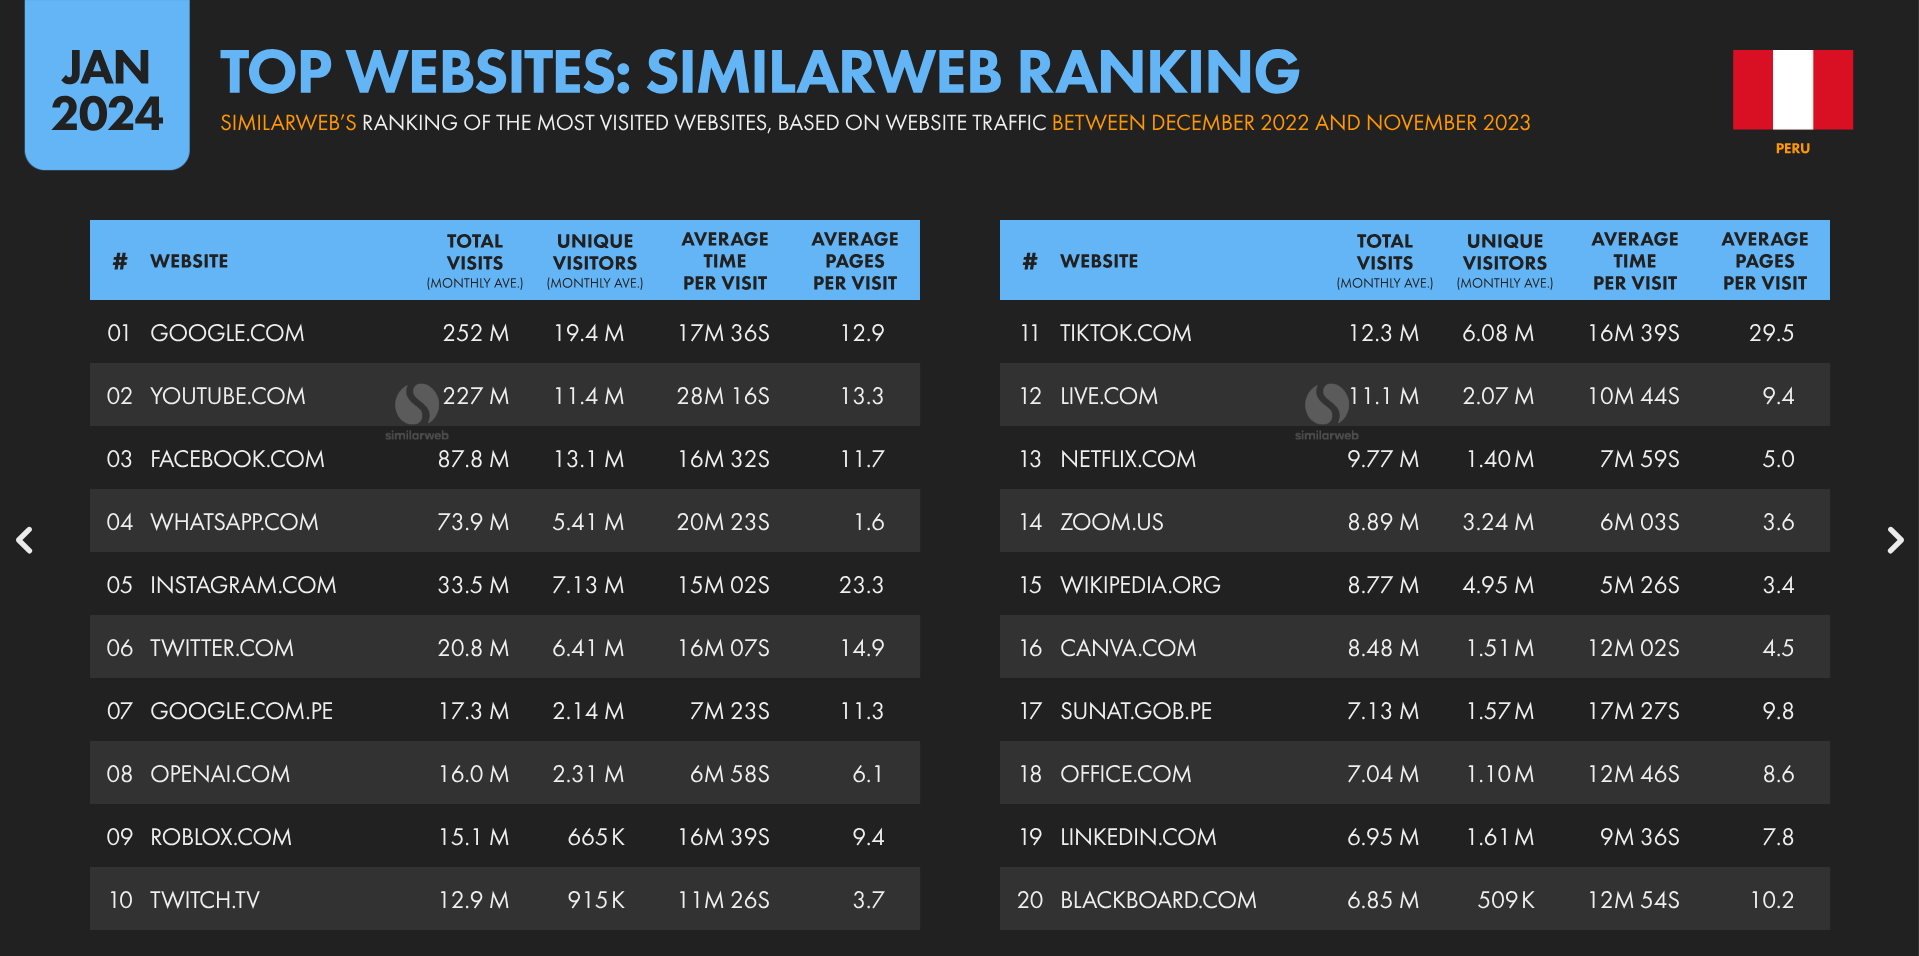
\includegraphics[width=0.80\textwidth]{1/figures/Top_Peru_2023.png}
	\caption[Top webs más visitadas en Perú en 2023]{Top webs más visitadas en Perú en 2023. \\ Fuente: \cite{youtube_peru}. \textit{Basado en el tráfico web de Diciembre de 2022 a Noviembre del 2023}.}
	\label{2:fig}
\end{figure}

Esta automatización optimiza tanto el tiempo como los recursos necesarios para curar contenido, mejorando la precisión en la selección de información significativa.

La generación de clips informativos a partir de videos largos presenta múltiples beneficios para los medios de comunicación. Primero, facilita la creación de resúmenes concisos y precisos que destacan los puntos clave de las noticias, permitiendo a los usuarios acceder a la información relevante de manera rápida. Este enfoque es crucial en un entorno donde la atención del usuario es limitada y la demanda de contenido digerible es alta.
Esto no solo aumenta el alcance y el impacto de las noticias, sino que también mejora la participación del público y fomenta una mayor interacción con el contenido.

La automatización en la generación de clips también contribuye a la eficiencia operativa de los medios. Al reducir la necesidad de intervención manual en la selección y edición de contenido, los recursos se liberan para enfocarse en otras áreas críticas, como la investigación y el análisis en profundidad. Esto permite a los medios mantenerse competitivos en un entorno en constante cambio y con una demanda creciente de contenido actualizado y relevante.


\subsection{Problema General}
\newcommand{\ProblemaGeneral}{
	¿De qué manera el desarrollo de una herramienta inteligente basada en técnicas de clustering de frames puede facilitar la identificación automática de tendencias a partir de videos de noticias para crear clips de videos representativos?}
\ProblemaGeneral
\subsection{Problemas Espec\'{i}ficos}
\newcommand{\Pbone}{¿Cómo obtener de manera eficiente los videos de noticias referentes a un día en específico, asegurando que sean representativos de los eventos más importantes del día?}
\newcommand{\Pbtwo}{¿Qué técnicas de preprocesamiento de imágenes y normalización son más efectivas para mejorar la calidad y relevancia de los frames extraídos de los videos?}
\newcommand{\Pbthree}{¿Qué técnicas de extracción de características permiten representar adecuadamente los frames para identificar patrones visuales relevantes?}
\newcommand{\Pbfour}{¿Cuál es el algoritmo de clustering más adecuado para agrupar los frames en base a las similitudes de las características extraídas que posean entre ellas?}
\newcommand{\Pbfive}{¿Cómo generar clips informativos concisos, asegurando que reflejen los eventos clave discutidos en las noticias?}

\begin{itemize}
	\item \Pbone
	\item \Pbtwo
	\item \Pbthree
	\item \Pbfour
	\item \Pbfive
\end{itemize}

\section{Objetivos de la Investigación}
\subsection{Objetivo General}
\newcommand{\ObjetivoGeneral}{
	Desarrollar una herramienta inteligente que identifique de manera automática tendencias en videos de noticias mediante el clustering de frames representativos y genere clips de videos que resuman los eventos clave.
}
\ObjetivoGeneral

\subsection{Objetivos Espec\'{i}ficos}
\newcommand{\Objone}{
	Desarrollar un método eficiente para la recolección de videos de noticias, asegurando que estos reflejen los eventos más importantes del día.
}
\newcommand{\Objtwo}{
	Implementar técnicas de preprocesamiento de imágenes y normalización que mejoren la calidad de los frames extraídos, optimizando su relevancia para el análisis.
}
\newcommand{\Objthree}{
	Desarrollar técnicas de extracción de características que permitan representar adecuadamente los frames, facilitando la identificación de patrones visuales relevantes.
}
\newcommand{\Objtfour}{
	Seleccionar e implementar un algoritmo de clustering que agrupe los frames basándose en la similitud de características, garantizando que los grupos formados representen tendencias claras.
}
\newcommand{\Objtfive}{
	Desarrollar un sistema automatizado para generar clips informativos concisos que resuman los eventos clave identificados en los videos de noticias.
}


\begin{itemize}
	\item {\Objone}
	\item {\Objtwo}
	\item {\Objthree}
	\item {\Objtfour}
	\item {\Objtfive}
\end{itemize}

\section{Justificación de la Investigación}

\subsection{Teórica}Esta investigación se realiza para determinar cómo el uso de herramientas de Big Data y modelos de aprendizaje automático puede optimizar la selección y generación de clips informativos concisos a partir de contenido audiovisual en YouTube. La teorización se centra en la capacidad de estas herramientas para manejar la sobrecarga de información y mejorar la eficiencia operativa en el proceso de curación de contenido. Este estudio contribuirá al cuerpo de conocimiento en el campo del análisis automatizado de contenido audiovisual, proponiendo un marco teórico para la implementación de tecnologías avanzadas en la industria de los medios de comunicación.
\subsection{Práctica}
Al culminar la investigación, se espera que los medios de comunicación puedan utilizar el sistema automatizado basado en Big Data y aprendizaje automático para seleccionar y generar clips informativos relevantes de manera eficiente. Esto facilitará la creación de resúmenes concisos que destaquen los puntos clave de las noticias, permitiendo a los usuarios acceder a información relevante rápidamente. La implementación práctica de esta solución tecnológica ayudará a los medios a adaptarse a las nuevas tendencias de consumo de contenido, donde la rapidez y concisión son cruciales. Además, mejorará la participación del público y fomentará una mayor interacción con el contenido.
\subsection{Metodológica}. 
El desarrollo del sistema automatizado de análisis de contenido audiovisual utilizando herramientas de Big Data y aprendizaje automático permitirá manejar grandes volúmenes de datos de video de manera eficiente. La metodología incluye el uso de PySpark para la gestión de datos distribuidos y técnicas de procesamiento de imágenes para la extracción de frames significativos. La implementación de algoritmos de clustering ayudará a identificar patrones y eventos relevantes. Esta metodología no solo optimiza el tiempo y los recursos necesarios para curar contenido, sino que también mejora la precisión en la selección de información significativa, ofreciendo una solución tecnológica avanzada para los desafíos actuales en el análisis de contenido audiovisual.
\section{Delimitación del Estudio}

\subsection{Espacial}
El estudio se llevará a cabo en el contexto de plataformas de redes sociales, enfocándose específicamente en YouTube como la principal fuente de contenido audiovisual para el análisis. Se seleccionarán videos de noticias y eventos actuales relevantes para el público peruano, dado que YouTube es una de las páginas más visitadas en Perú, con un alto volumen de visitas mensuales y visitantes únicos. La investigación se centrará en la capacidad de YouTube para proporcionar tanto contenido audiovisual como metadatos valiosos para el análisis.
\subsection{Temporal}
Los datos que se extraerán serán de la primera semana de Agosto del 2024, se realizará la recopilación, procesamiento y análisis. Al ser una herramienta de uso periódico, los resultados se generarán minutos posteriores a la culminación del proceso de recopilación.
\subsection{Conceptual}
La presente investigación se centrará en el desarrollo de un sistema automatizado para la selección y generación de clips informativos a partir de contenido audiovisual utilizando herramientas de Big Data y modelos de aprendizaje automático. El enfoque estará en el análisis de videos de noticias en YouTube, aplicando técnicas de procesamiento de imágenes y algoritmos de clustering para identificar eventos relevantes.
\section{Hipótesis}

\subsection{Hipótesis General}
\newcommand{\HipotesisGeneral}{
	Mediante el uso de técnicas de modelos de aprendizaje automático, se logrará mejorar la identificación de tendencias y la generación de clips informativos representativos de videos de noticias.
}
\HipotesisGeneral

\HipotesisGeneral
\subsection{Hipótesis Específicas}
\newcommand{\Hone}{
	La recolección automatizada de videos de noticias referentes a un día específico permitirá capturar de manera eficiente los contenidos más representativos para el análisis de tendencias.
}
\newcommand{\Htwo}{
	El uso de técnicas avanzadas de preprocesamiento y normalización de imágenes mejorará significativamente la calidad de los frames, facilitando su clasificación y análisis posterior.
}
\newcommand{\Hthree}{
	La extracción de características adecuadas de los frames permitirá identificar correctamente patrones visuales que reflejen temas importantes y eventos clave.
}
\newcommand{\Hfour}{
	El uso de un algoritmo de clustering optimizado permitirá agrupar los frames con precisión en función de sus similitudes, identificando adecuadamente las tendencias en los noticias.
}
\newcommand{\Hfive}{
	La generación automatizada de clips informativos basados en las tendencias identificadas ofrecerá resúmenes concisos y efectivos de los eventos más relevantes del día.
}
\begin{itemize}
	\item \Hone
	\item \Htwo
	\item \Hthree
	\item \Hfour
	\item \Hfive
\end{itemize}

\subsection{Matriz de Consistencia}
A continuación se presenta la matriz de consistencia elaborada para la presente investigación (véase Anexo \ref{1:table}).

